\chapter{拉格朗日乘数}
微积分中最常见的问题之一是求一个函数的极大极小值(极值).但是很多时候找到极值函数的显式表达是很困难的,特别是当函数有先决条件或约束时.
拉格朗日乘数则提供了一个非常便利方法来解决这类问题,而避开显式地引入约束和求解外部变量.

\section{Theory}
\begin{figure}[htbp]
  \centering
  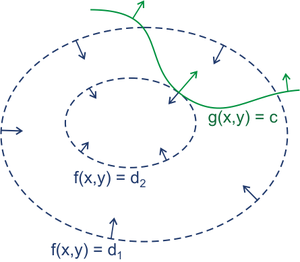
\includegraphics[scale = 0.5]{Lagrange_multiplier}\\
  \caption{Lagrange multiplier}
  \label{fig.Lagrange.multiplier}
\end{figure}

先看一个二维的例子:假设有函数:$f(x, y)$,要求其极值(最大值/最小值),且满足条件
$$ g\left( x,y \right) = 0, $$
c 为常数.对不同$d_n$的值,不难想像出

$$ f \left( x, y \right)=d_n $$
的等高线, 如图\ref{fig.Lagrange.multiplier},
\href{http://upload.wikimedia.org/wikipedia/commons/thumb/f/fa/Lagrange\_multiplier.png/300px-Lagrange\_multiplier.png}{Lagrange multiplier}所示.

假设g(x)与等高线相交,交点就是同时满足等式约束条件和目标函数的可行域的值,但肯定不是最优值,
因为相交意味着肯定还存在其它的等高线在该条等高线的内部或者外部,使得新的等高线与目标函数的交点的值更大或者更小,
只有到等高线与目标函数的曲线相切的时候,可能取得最优值(最大值或者最小值, 图中所示为最大值),
即等高线和目标函数的曲线在该点的法向量必须有相同方向,
所以最优值必须满足:f(x)的梯度 = a* g(x)的梯度,a是常数,表示左右两边同向.
这个等式就是L(a,x)对参数求导的结果

而方程 g 的可行集所构成的线正好是 $g ( x, y ) = c$ .想像我们沿着 $g = c$ 的可行集走,
因为大部分情况下 f 的等高线和 g 的可行集线不会重合,但在有解的情况下,这两条线会相交.想像此时我们移动 $g = c$ 上的点,因为 f 是连续的方程,
我们因此能走到$f \left( x, y \right)=d_n$更高或更低的等高线上,也就是说$d_n$可以变大或变小.只有当 $g = c$ 和$f \left( x, y \right)=d_n$相切,也就是说,
此时,我们正同时沿着 $g = c$ 和$f \left( x, y \right)=d_n$走.这种情况下,会出现极值或鞍点.

用向量的形式来表达的话,我们说相切的性质在此意味着 f 和 g 的切线在某点上平行.此时引入一个未知标量$\lambda$,并求解:

$$ \nabla \Big[f \left(x, y \right) + \lambda \left(g \left(x, y \right) - c \right) \Big] = 0 $$
且$\lambda \neq 0$.

一旦求出$\lambda$的值,将其套入下式,易求在无约束极值和极值所对应的点.

$$ F \left( x , y \right)  =  f \left( x , y \right) + \lambda \left( g \left( x , y \right) - c \right) $$
新方程$F(x,y)$在达到极值时与$f(x,y)$相等,因为$F(x,y)$达到极值时$g(x,y)-c$总等于零.

\section{Example}
\begin{example}
\textbf{求方程的最小值}:

$$ f(x, y) = x^2 y $$
同时未知数满足

$$ x^2 + y^2 = 1 $$
因为只有一个未知数的限制条件,我们只需要用一个乘数$\lambda$.

$$
\begin{aligned}
		& g (x, y) = x^2 +y^2 -1 \\
		& \Phi (x, y, \lambda) = f(x,y) + \lambda g(x, y) = x^2 y + \lambda (x^2 + y^2 - 1)
\end{aligned}
$$
将所有$\Phi$方程的偏微分设为零,得到一个方程组,最大值是以下方程组的解中的一个:

$$
\begin{aligned}
		& 2 x y + 2 \lambda x = 0 \\
		& x^2 + 2 \lambda y = 0 \\
		& x^2 + y^2 -1 = 0
\end{aligned}
$$
求解方程组,结果
\end{example}

\begin{example}
\textbf{离散分布的最大熵}:

$$ f(p_1,p_2,\ldots,p_n) = -\sum_{k=1}^n p_k\log_2 p_k.  $$
所有概率的总和是1,因此我们得到的约束是$g(p)= 1$即

$$ g(p_1,p_2,\ldots,p_n)=\sum_{k=1}^n p_k=1.  $$
可以使用拉格朗日乘数找到最高熵(概率的函数).对于所有的k 从1到n,要求

$$ \frac{\partial}{\partial p_k}(f+\lambda (g-1))=0, $$
由此得到

$$ \frac{\partial}{\partial p_k}\left(-\sum_{k=1}^n p_k \log_2 p_k + \lambda (\sum_{k=1}^n p_k - 1) \right) = 0.  $$
计算出这n个等式的微分,我们得到:

$$ -\left(\frac{1}{\ln 2}+\log_2 p_k \right) + \lambda = 0.  $$
这说明$p_i$都相等 (因为它们都只是$\lambda$的函数). 解出约束$\sum_k p_k = 1$,得到

$$ p_k = \frac{1}{n}.$$
因此,使用均匀分布可得到最大熵的值.
\end{example}

\section{KKT条件}
在满 足一些有规则的条件下,一个非线性规划(Nonlinear Programming)问题能有最优化解法的一个必要和充分条件.这是一个广义化拉格朗日乘数的成果.

考虑以下非线式最优化问题:
$$
\begin{aligned}
& \min\limits_{x}\;\; f(x) \\
& \mbox{Subject to: } g_i(x) \le 0 , h_j(x) = 0
\end{aligned}
$$
$f(x)$是需要最小化的函数,
$g_i (x)\ (i = 1, \ldots,m)$是不等式约束,
$h_j (x)\ (j = 1,\ldots,l)$是等式约束,
$m$和$l$分别为不等式约束和等式约束的数量.

把所有的不等式约束,等式约束和目标函数全部写为一个式子
$L(a, b, x)= f(x) + a*g(x)+b*h(x)$,
KKT条件是说最优值必须满足以下条件:

\begin{enumerate}
\item $L(a, b, x)$对x求导为零,
\item $h(x) =0$;
\item $a*g(x) = 0$;
\end{enumerate}
其中$a, h, g$都是向量表达形式

求取这三个等式之后就能得到候选最优值.其中第三个式子非常有趣, 因为
$g(x)<=0$,如果要满足第三个等式,必须$a=0$或者$g(x)=0$.\\
这是SVM的很多重要性质的来源,如支持向量的概念

而KKT条件是满足强对偶条件的优化问题的必要条件,可以这样理解:我们要求$min f(x), L(a, b, x) = f(x) + a*g(x) + b*h(x),a>=0$,
我们可以把$f(x)$写为:$max_{a,b} L(a,b,x)$,为什么呢?因为$h(x)=0, g(x)<=0$,现在是取$L(a,b,x)$的最大值,$a*g(x)<=0$,
所以$L(a,b,x)$只有在$a*g(x) = 0$的情况下才能取得最大值,否则,就不满足约束条件,
因此m$ax_{a,b} L(a,b,x)$在满足约束条件的情况下就是$f(x)$,因此我们的目标函数可以写为 $min_x max_{a,b} L(a,b,x)$.\\
如果用对偶表达式: $max_{a,b} min_x  L(a,b,x)$,由于我们的优化是满足强对偶的(强对偶就是说对偶式子的最优值是等于原问题的最优值的),
所以在取得最优值$x0$的条件下,它满足$f(x0) = max_{a,b} min_x  L(a,b,x) = min_x max_{a,b} L(a,b,x) =f(x0)$,我们来看看中间两个式子发生了什么事情:
$$ f(x0) = max_{a,b} min_x  L(a,b,x) =  max_{a,b} min_x f(x) + a*g(x) + b*h(x) =  max_{a,b} f(x0)+a*g(x0)+b*h(x0) = f(x0) $$

可以看到上述加黑的地方本质上是说 $min_x f(x) + a*g(x) + b*h(x)$ 在$x0$取得了最小值,用fermat定理,即是说对于函数 $f(x) + a*g(x) + b*h(x)$,求取导数要等于零,即

$$ f(x)的梯度+a*g(x)的梯度+ b*h(x)的梯度 = 0 $$

这就是kkt条件中第一个条件:$L(a, b, x)$对$x$求导为零.

而之前说明过,$a*g(x) = 0$,这时kkt条件的第3个条件,当然已知的条件$h(x)=0$必须被满足,
所有上述说明,满足强对偶条件的优化问题的最优值都必须满足KKT条件,即上述说明的三个条件.\\
可以把KKT条件视为是拉格朗日乘子法的泛化.

